%%%%%%%%%%%%%%%%%%%%%%%%%%%%%%%%%%%%%%%%%%%%%%%%%%%%%%%%%%%%%%%%%%%%%%%%%%%%%%%%%
%% Documenclass 
%%%%%%%%%%%%%%%%%%%%%%%%%%%%%%%%%%%%%%%%%%%%%%%%%%%%%%%%%%%%%%%%%%%%%%%%%%%%%%%%%
\documentclass[a4paper,oneside,titlepage]{report}
%%%%%%%%%%%%%%%%%%%%%%%%%%%%%%%%%%%%%%%%%%%%%%%%%%%%%%%%%%%%%%%%%%%%%%%%%%%%%%%%%
%% Packages
%%%%%%%%%%%%%%%%%%%%%%%%%%%%%%%%%%%%%%%%%%%%%%%%%%%%%%%%%%%%%%%%%%%%%%%%%%%%%%%%%
\usepackage[english]{babel}
\usepackage{amsmath}
\usepackage{complexity}
\usepackage[T1]{fontenc}
\usepackage[utf8]{inputenc}
\usepackage[pdftex]{graphicx} %%Graphics in pdfLaTeX
\usepackage{a4wide} %%Smaller margins, more text per page.
\usepackage{longtable} %%For tables that exceed a page width
\usepackage{pdflscape} %%Adds PDF sup­port to the land­scape en­vi­ron­ment of pack­age
\usepackage{caption} %%Pro­vides many ways to cus­tomise the cap­tions in float­ing en­vi­ron­ments like fig­ure and ta­ble
\usepackage{float} %%Im­proves the in­ter­face for defin­ing float­ing ob­jects such as fig­ures and ta­bles
\usepackage[tablegrid,nochapter]{vhistory} %%Vhis­tory sim­pli­fies the cre­ation of a his­tory of ver­sions of a doc­u­ment
\usepackage[nottoc]{tocbibind} %%Au­to­mat­i­cally adds the bib­li­og­ra­phy and/or the in­dex and/or the con­tents, etc., to the Ta­ble of Con­tents list­ing
\usepackage[toc,page]{appendix} %%The ap­pendix pack­age pro­vides var­i­ous ways of for­mat­ting the ti­tles of ap­pen­dices
\usepackage{pdfpages} %%This pack­age sim­pli­fies the in­clu­sion of ex­ter­nal multi-page PDF doc­u­ments in LATEX doc­u­ments
\usepackage[rightcaption]{sidecap} %%De­fines en­vi­ron­ments called SC­fig­ure and SCtable (anal­o­gous to fig­ure and ta­ble) to type­set cap­tions side­ways
\usepackage{cite} %%The pack­age sup­ports com­pressed, sorted lists of nu­mer­i­cal ci­ta­tions, and also deals with var­i­ous punc­tu­a­tion and other is­sues of rep­re­sen­ta­tion, in­clud­ing com­pre­hen­sive man­age­ment of break points
\usepackage[]{acronym} %%This pack­age en­sures that all acronyms used in the text are spelled out in full at least once. It also pro­vides an en­vi­ron­ment to build a list of acronyms used
\usepackage[pdftex,scale={.8,.8}]{geometry} %%The pack­age pro­vides an easy and flex­i­ble user in­ter­face to cus­tomize page lay­out, im­ple­ment­ing auto-cen­ter­ing and auto-bal­anc­ing mech­a­nisms so that the users have only to give the least de­scrip­tion for the page lay­out. For ex­am­ple, if you want to set each mar­gin 2cm with­out header space, what you need is just \usep­a­ck­age[mar­gin=2cm,no­head]{ge­om­e­try}.
\usepackage{layout} %%The pack­age de­fines a com­mand \lay­out, which will show a sum­mary of the lay­out of the cur­rent doc­u­ment
\usepackage{subfigure} %%Pro­vides sup­port for the ma­nip­u­la­tion and ref­er­ence of small or ‘sub’ fig­ures and ta­bles within a sin­gle fig­ure or ta­ble en­vi­ron­ment.
\usepackage[toc]{glossaries} %%The glos­saries pack­age sup­ports acronyms and mul­ti­ple glos­saries, and has pro­vi­sion for op­er­a­tion in sev­eral lan­guages (us­ing the fa­cil­i­ties of ei­ther ba­bel or poly­glos­sia).
\usepackage[left,pagewise,modulo]{lineno} %%Adds line num­bers to se­lected para­graphs with ref­er­ence pos­si­ble through the LATEX \ref and \pageref cross ref­er­ence mech­a­nism
\usepackage[pdftex,colorlinks=false,hidelinks,pdfstartview=FitV]{hyperref}%%The hy­per­ref pack­age is used to han­dle cross-ref­er­enc­ing com­mands in LATEX to pro­duce hy­per­text links in the doc­u­ment. 
\usepackage{metainfo}
\usepackage[pagestyles,raggedright]{titlesec}
\usepackage{etoolbox}
\usepackage{%
	array, %%An ex­tended im­ple­men­ta­tion of the ar­ray and tab­u­lar en­vi­ron­ments which ex­tends the op­tions for col­umn for­mats, and pro­vides "pro­grammable" for­mat spec­i­fi­ca­tions
	booktabs, %%The pack­age en­hances the qual­ity of ta­bles in LATEX, pro­vid­ing ex­tra com­mands as well as be­hind-the-scenes op­ti­mi­sa­tion
	dcolumn, %%
	rotating,
	shortvrb,
	units,
	url,
	lastpage,
	longtable,
	lscape,
	qtree,
	skmath,	
}
%%%%%%%%%%%%%%%%%%%%%%%%%%%%%%%%%%%%%%%%%%%%%%%%%%%%%%%%%%%%%%%%%%%%%%%%%%%%%%%%%
%% Java --> latex 
%%%%%%%%%%%%%%%%%%%%%%%%%%%%%%%%%%%%%%%%%%%%%%%%%%%%%%%%%%%%%%%%%%%%%%%%%%%%%%%%%
\usepackage{listings}
\usepackage{color}
\definecolor{pblue}{rgb}{0.13,0.13,1}
\definecolor{pgreen}{rgb}{0,0.5,0}
\definecolor{pred}{rgb}{0.9,0,0}
\definecolor{pgrey}{rgb}{0.46,0.45,0.48}
\usepackage{inconsolata}
%%Listing style for java.
\definecolor{dkgreen}{rgb}{0,0.6,0}
\definecolor{gray}{rgb}{0.5,0.5,0.5}
\definecolor{mauve}{rgb}{0.58,0,0.82}
\lstset{frame=tb,
	language=Java,
	aboveskip=3mm,
	belowskip=3mm,
	showstringspaces=false,
	columns=flexible,
	basicstyle={\small\ttfamily},
	numbers=left,
	numberstyle=\tiny\color{gray},
	keywordstyle=\color{blue},
	commentstyle=\color{dkgreen},
	stringstyle=\color{mauve},
	breaklines=true,
	breakatwhitespace=true,
	tabsize=3
}

%%%%%%%%%%%%%%%%%%%%%%%%%%%%%%%%%%%%%%%%%%%%%%%%%%%%%%%%%%%%%%%%%%%%%%%%%%%%%%%%%
\setlength{\parindent}{0pt}
\setlength{\parskip}{.5\baselineskip}
%%%%%%%%%%%%%%%%%%%%%%%%%%%%%%%%%%%%%%%%%%%%%%%%%%%%%%%%%%%%%%%%%%%%%%%%%%%%%%%%%
%% Inserting the metadata
%%%%%%%%%%%%%%%%%%%%%%%%%%%%%%%%%%%%%%%%%%%%%%%%%%%%%%%%%%%%%%%%%%%%%%%%%%%%%%%%%
% % Metadaten des Dokumentes

\usepackage{graphicx}

\titleformat{\chapter}[display]
  {\normalfont\bfseries}{}{0pt}{\Huge}

\def\Company{Institution}
\def\Institute{\textit{National Institute of Technology, Calicut}}
\def\Course{\textit{Computer Science and Enginnering}}
\def\Module{\textit{Bachelor of Technology (BTech)}}
\def\Docent{\textit{Software Engineering (CS3004D)}}
\def\Assistant{\textit{Somone}}

\def\BoldTitle{Software Requirements Specification}

\def\Subtitle{for \\ Institute Firewall Login Manager for Android \\}
\def\Authors{
Mohammed Shahraaz Hussain B170252CS B Batch \\
Ishan Ghosh B170473CS B Batch \\
Kapil Gyanchandani B170583CS B Batch\\
Vinay Kumar Saxena  B170338CS B Batch\\
Goutham Krishna K V B170214CS A Batch\\
} 

\title{\textbf{\BoldTitle}\\\Subtitle}
\author{\Authors \\ \\ \\ \Institute\\ \Course\\ \Module\\ \Docent\\} %\Assistant}
\date{January 2020}

%%%%%%%%%%%%%%%%%%%%%%%%%%%%%%%%%%%%%%%%%%%%%%%%%%%%%%%%%%%%%%%%%%%%%%%%%%%%%%%%%
%% Creation of pdf information
%%%%%%%%%%%%%%%%%%%%%%%%%%%%%%%%%%%%%%%%%%%%%%%%%%%%%%%%%%%%%%%%%%%%%%%%%%%%%%%%%
\hypersetup{pdfinfo={
		Title={Title},
		Author={TR},
		Subject={Report}
	}}
%%%%%%%%%%%%%%%%%%%%%%%%%%%%%%%%%%%%%%%%%%%%%%%%%%%%%%%%%%%%%%%%%%%%%%%%%%%%%%%%%
%% Creating the frontpage
%%%%%%%%%%%%%%%%%%%%%%%%%%%%%%%%%%%%%%%%%%%%%%%%%%%%%%%%%%%%%%%%%%%%%%%%%%%%%%%%%
\AtBeginDocument{
	\maketitle
	\thispagestyle{empty}
}

%%%%%%%%%%%%%%%%%%%%%%%%%%%%%%%%%%%%%%%%%%%%%%%%%%%%%%%%%%%%%%%%%%%%%%%%%%%%%%%%%
%% Creation of the header
%%%%%%%%%%%%%%%%%%%%%%%%%%%%%%%%%%%%%%%%%%%%%%%%%%%%%%%%%%%%%%%%%%%%%%%%%%%%%%%%%
\patchcmd{\chapter}{plain}{short}{}{} %$ <-- the header on chapter 1
%%%%%%%%%%%%%%%%%%%%%%%%%%%%%%%%%%%%%%%%%%%%%%%%%%%%%%%%%%%%%%%%%%%%%%%%%%%%%%%%%
%% Creation of page-styles
%%%%%%%%%%%%%%%%%%%%%%%%%%%%%%%%%%%%%%%%%%%%%%%%%%%%%%%%%%%%%%%%%%%%%%%%%%%%%%%%%
\newpagestyle{long}{%
	\sethead[\thepage][][\chaptername\ \thechapter:\ \chaptertitle]{\chaptername\ \thechapter:\ \chaptertitle}{}{\thepage}
	\headrule
}

\newpagestyle{short}{%
	\sethead[\thepage][][]{}{}{\thepage}
	\headrule
}
%%%%%%%%%%%%%%%%%%%%%%%%%%%%%%%%%%%%%%%%%%%%%%%%%%%%%%%%%%%%%%%%%%%%%%%%%%%%%%%%%
%% DOCUMENT
%%%%%%%%%%%%%%%%%%%%%%%%%%%%%%%%%%%%%%%%%%%%%%%%%%%%%%%%%%%%%%%%%%%%%%%%%%%%%%%%%
\begin{document}

\pagenumbering{roman}
\DeclareGraphicsExtensions{.pdf,.jpg,.png}
\pagestyle{short}



\newpage
%%%%%%%%%%%%%%%%%%%%%%%%%%%%%%%%%%%%%%%%%%%%%%%%%%%%%%%%%%%%%%%%%%%%%%%%%%%%%%%%%
%% Table of contents
%%%%%%%%%%%%%%%%%%%%%%%%%%%%%%%%%%%%%%%%%%%%%%%%%%%%%%%%%%%%%%%%%%%%%%%%%%%%%%%%%
 \tableofcontents % Inhaltsverzeichnis



\pagestyle{long}




%%%%%%%%%%%%%%%%%%%%%%%%%%%%%%%%%%%%%%%%%%%%%%%%%%%%%%%%%%%%%%%%%%%%%%%%%%%%%%%%%
%% Version table insertion
%%%%%%%%%%%%%%%%%%%%%%%%%%%%%%%%%%%%%%%%%%%%%%%%%%%%%%%%%%%%%%%%%%%%%%%%%%%%%%%%%
% Versionstabelle.

\chapter*{Revision History}
\addcontentsline{toc}{chapter}{Revision History}
\begin{versionhistory}
	\vhEntry{1.0}{22.01.2020}{All}{Revision 1}
    \vhEntry{2.0}{26.01.2020}{All}{Revision 2}
    \vhEntry{3.0}{27.01.2020}{All}{Revision 3}
    \vhEntry{4.0}{28.01.2020}{All}{Revision 4}
    %\vhEntry{4.0}{10.01.2016}{}{Finale Version}


\end{versionhistory}
\pagenumbering{arabic}
%%%%%%%%%%%%%%%%%%%%%%%%%%%%%%%%%%%%%%%%%%%%%%%%%%%%%%%%%%%%%%%%%%%%%%%%%%%%%%%%%
%% Inserting all the content
%%%%%%%%%%%%%%%%%%%%%%%%%%%%%%%%%%%%%%%%%%%%%%%%%%%%%%%%%%%%%%%%%%%%%%%%%%%%%%%%%
\chapter{Introduction}
\label{ch:intro}
\section{Purpose}
The purpose of this document is to capture, in natural language and a functional level, the description and requirements of a Institute Firewall Login Manager Application. The focus here is to automate the process of connecting to the institute network. This is a functional description of those features required to address the current network connectivity issue. A short discussion accompanies each requirement, to add the background and framework necessary to explain the functionality. It also describes nonfunctional requirements and other factors necessary to provide a complete and comprehensive description of the requirements for the software. 
\section{Document Conventions}
This document was created based on the IEEE template for System Requirement Specification Documents.

Abbreviations:
\begin{itemize}
    \item FLMI: Firewall Login Manager for Institutes.
    \item WiFi: Wireless Fidelity, a local area wireless network. 
    \item FOSS: Free and Open Source Software
    \item UI: User interface.
    \item URL: Uniform Resource Locator.
    \item CNC: Campus Networking Center.
\end{itemize}


\section{Intended Audience and Reading Suggestions}
This Software Requirements document is intended for:
\begin{itemize}
    \item Developers who can review project’s capabilities and more  easily  understand  where  their efforts  should  be targeted to improve or add more features to it (design and code of the application. It  sets  the  guidelines  for  future development).
    \item Project testers can use this document as a base for their testing  strategy  as  some  bugs  are easier  to  find  using  a requirements  document.  This  way  testing  becomes  more methodically organized.
    \item End  users  of  this  application  who  wish  to  read  about what this project can do.
\end{itemize}
\section{Product Scope}
Institutes all over the country use a firewall to allow only institute members to use the campus network. This Login Manager has two internal scopes, one dealing with the details of the user account and second dealing with the Institute Firewall.

\subsection{Objectives}
\begin{itemize}
    \item Automate the login and logout process for connecting to the campus network.
    \item Reduce delay and number of steps.
    \item Store User Account details.
    \item Reduce Keep-alive errors.
\end{itemize}

\subsection{Expectations}
\begin{itemize}
    \item Only one time entry of the user Account details required.
    \item Use only a single button to toggle between login and logout states.
\end{itemize}

\subsection{Constraints}
\begin{itemize}
    \item The user upon leaving the network before logging out, is then locked from another login for 40 minutes or until he is connected to the same network.
    \item When the network breaks down the application will stop functioning. 
\end{itemize}

\section{References}
\begin{itemize}
    \item IEEE SRS template: \\ \texttt{https://www.overleaf.com/latex/templates/requirements-specification-layout/vbrqbjpzcmfy}
    \item GitHub Project Link: \texttt{https://github.com/Shahraaz/LoginManager}
    \item Wikipedia: \texttt{https://www.wikipedia.org/}
    \item Use Case Diagram: \texttt{https://www.draw.io/}
\end{itemize}


\chapter{Overall Description}
\label{Overall Description}

\section{Product Perspective}
FLMI serves as an automation tool for connecting to the campus network. It strives to eliminate the need to enter the user details, which is the username and password of a student or a member of the institute manually. FLMI also reduces the multiple steps required to authenticate and login to the campus firewall network. The application aims to remove user-generated issues such as the loss of the Keepalive window, forget passwords.
The application helps secure connectivity and worry-free access to the campus network. FLMI works on all mobile devices which run on the Android operating system.

\section{Product Features}
FLMI provides users the following features:
\begin{itemize}
    \item Detect IP address and magic number: The application detects the IP address of the router of the WiFi network to which the mobile device is connected and receives the webpage containing the firewall portal. 
    \item Login: One tap of a button can log the user into a connected network. 
    \item Logout: The user can logout of a already logged in network using a button.
    \item Keepalive: The login of a user is maintained continuously by re-sending login requests after Keepalive time has expired. 
    \item Add, Delete or Edit multiple user accounts: Multiple usernames and passwords for connecting to the firewall can be stored in the database of the application.
    \item Set credentials preferences: Most recently used Account is stored as next account to be used for login.
    \item Log Keepalive history: User login history is stored in the database so if a user forgets to logout of a network he can know to which network he was last connected.
\end{itemize}

\subsection{Use Case Diagrams}
\subsubsection{Overall Systems}
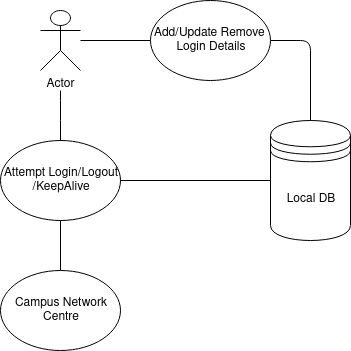
\includegraphics[scale=0.7]{images/final.png}

\subsubsection{Fetch IP Address and Magic Number}
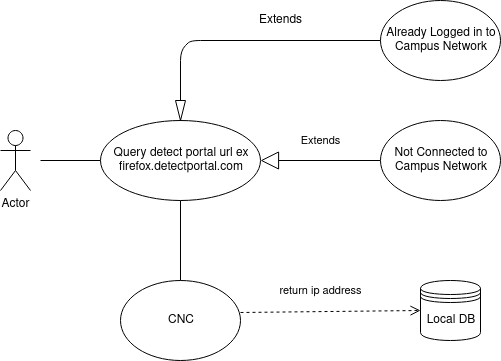
\includegraphics[scale=0.7]{images/ip.png}

\subsubsection{Login}
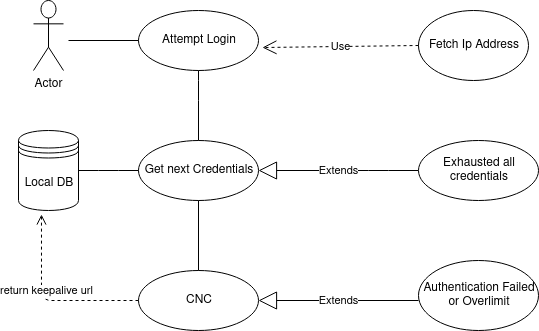
\includegraphics[scale=0.7]{images/login.png}

\subsubsection{Logout}
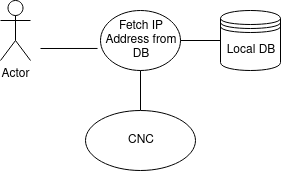
\includegraphics[scale=0.7]{images/Logout.png}

\subsubsection{Add or Remove Users}
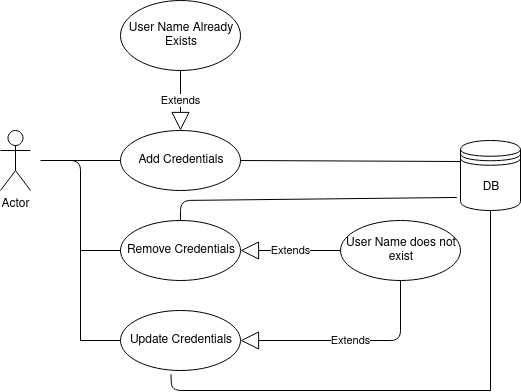
\includegraphics[scale=0.7]{images/add.png}

\subsection{Data Flow Diagram for login}
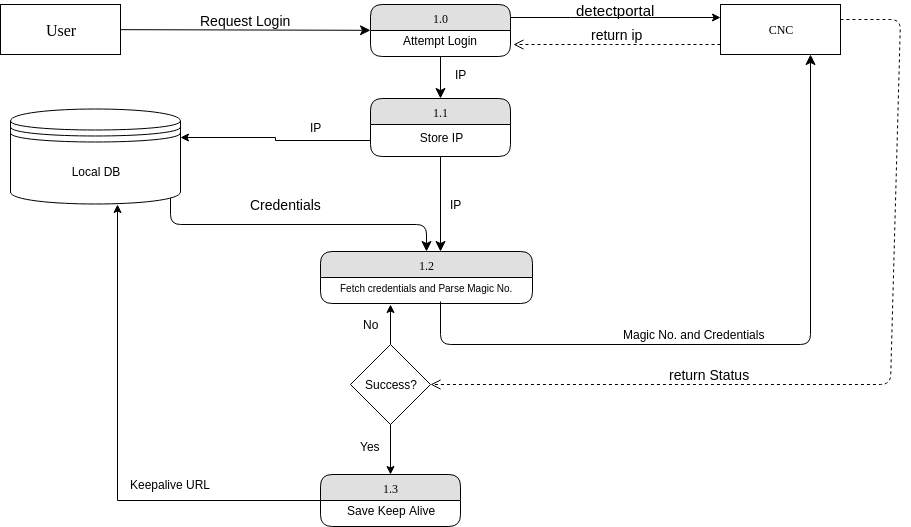
\includegraphics[width=\textwidth]{images/dfd.png}

\section{User Classes and Characteristics}

\begin{itemize}
    \item All kind of users: FLMI is a very simple to use application, all users with basic experience with technology are able to use it efficiently.
    \item Open source software developers and contributors: 
        \begin{itemize}
            \item Software developers: People with very good knowledge of the programming language, the project, in order to understand and be able to extend project's source code.
            \item Anyone who wants to help the FOSS community. The whole project is based on the conception of Free and Open Source Software, so all people are welcome to contribute any way they can/like.
        \end{itemize}
\end{itemize}

\section{Operating Environment}
FLMI requires an Android OS mobile device. An android device that can support basic dependencies of the application is expected for proper user experience.

\section{Design and Implementation Constraints}
FLMI is under the GNU General Public License Version 3.0, 2007. Everyone, that does or is going to develop or use FLMI, should agree and fully accept the terms of this kind of license. 

\section{User Documentation}
Any issues or questions related to the software can be asked by raising an issue on the github page of FLMI.
\href{https://github.com/Shahraaz/LoginManager}{\texttt{https://github.com/Shahraaz/LoginManager}}

\section{Assumptions and Dependencies}
FLMI is an android application it requires and mobile Android device to run. The Apk file has to be downloaded and installed on the device. Proper permissions should be granted when requested to the user to ensure the full functionality of the application. 

The device should be connected to a strong WiFi network with a firewall only then can the login and logout functionality be used. The device, once logged in from one network, cannot be logged out on another network.

\newpage
\chapter{External Interface Requirements}
\label{External Interface Requirements}

\section{User Interfaces}

Using the application is relatively simple and intuitive. A user familiar with the primary android application interface and navigation skill should be able to understand all functionality provided by the application. Nothing additional is required.

\section{Hardware Interfaces}
The application should work on mobile devices which are based on the Android operating system. No additional hardware interfaces required.

\section{Software Interfaces}
The application should run on Android 5.0 and above. Android below 5.0 (Lolipop) might cause some undefined behavior. The android device should have the application installed and proper permissions granted. It should also have the ability to connect to a WiFi network using the system hardware. 

\section{Data Management Interfaces}
The application should be able to interact with other components in the android device according to their specifications. Its operating device also limits the application in terms of the maximum number of user accounts the device's database can store at a particular time.

The tables in the database are as follows:\\
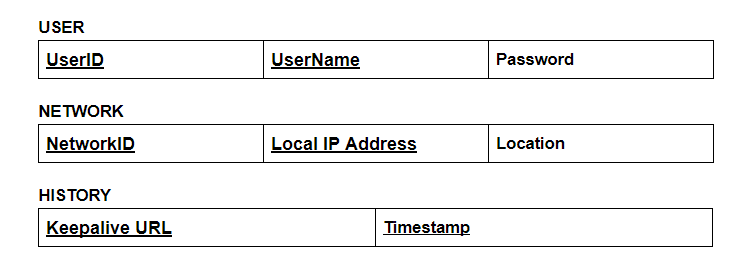
\includegraphics[scale=0.7]{images/table.png}

\section{Communications Interfaces}
There is a requirement of a working WiFi connection with a firewall setup and a valid user account in that firewall to use all of the functionality of the application. Additionally, an internet connection is required to download the application and update it. The only functionality available offline is the ability of the user to add multiple accounts and change passwords of an account.

\chapter{System Features}
\label{System Features}
The Priority ranges from 1 (most important) to 10 (least important).


\section{Fetch IP Address and Magic Number}
\subsection{Description and Priority}
The device would request a detect portal request though the Network. The network sends back a firewall login page back to the device requested.
Priority = 1.

\subsection{Functional Requirements}
\begin{itemize}
    \item \textbf{Purpose} : The IP address indicates which network the user is connected to and the magic number indicates currently which user is connected to which network.
    \item \textbf{User} : The application sends a request.
    \item \textbf{Input Data}: request to detectportal.firefox.com.
    \item \textbf{Output Data}: Corresponding Page Data.
    \item \textbf{Invariants}: Device is connected to a network.
    \item \textbf{Pre-conditions}: The mobile device is not logged in to the network.
    \item \textbf{Post-conditions}: The page data of the firewall portal is sent to the application
    \item \textbf{Basic Flow}: The application sends a request for the firewall portal from the mobile device the firewall if the device is not already logged in to the network sends back data regarding the firewall portal page.
    \item \textbf{Alternative Flow(s)}: If the device is already logged in to the network the request doesn't return back anything.
    \item \textbf{Business Rules}: This allows the user to access the login portal.
\end{itemize}

\section{Login}
\subsection{Description and Priority}
The system sends a login request to the network portal. The network portal, upon receiving this then responds with either a keepalive page (indicating that the user was logged in) or with another login (indicating that the user wasn't authenticated).
Priority = 1. \\

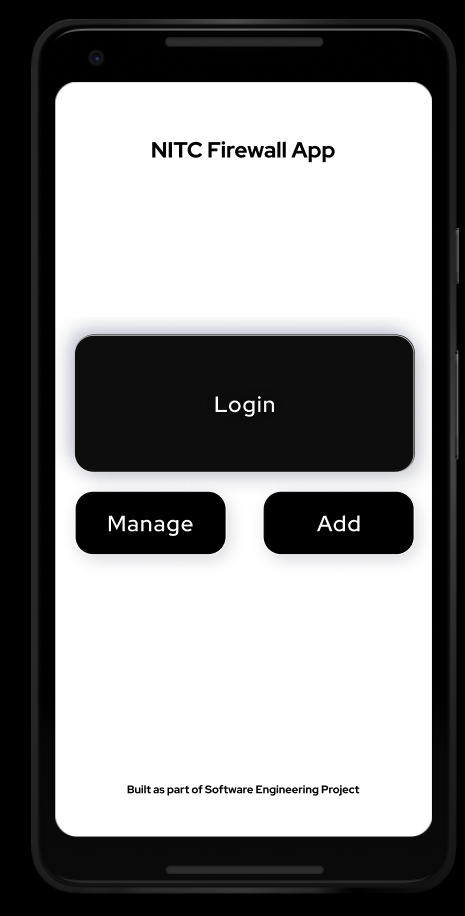
\includegraphics[scale=0.3]{images/hello.png} \\

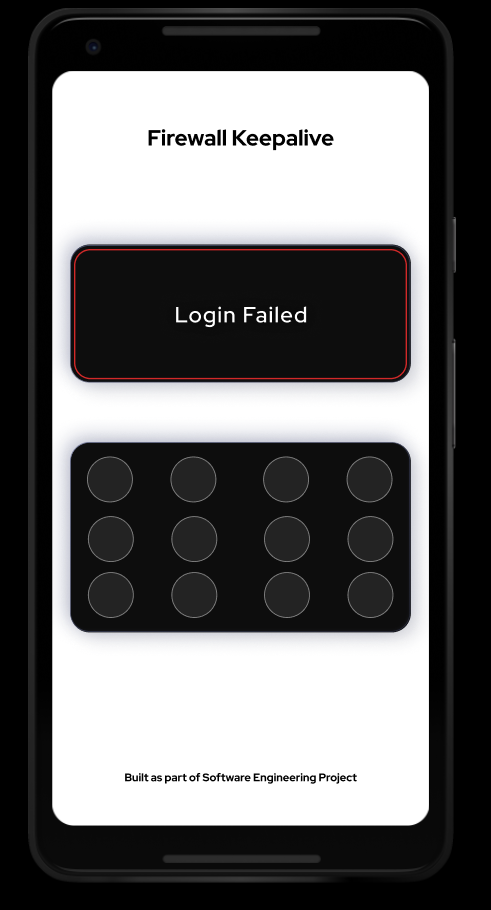
\includegraphics[scale=0.3]{images/hello3.png}
\subsection{Functional Requirements}
\begin{itemize}
    \item \textbf{Purpose}: Give the user rights to access the internet.
    \item \textbf{Input Data}: Valid user details.
    \item \textbf{Output Data}: KeepAlive Page data of the firewall.
    \item \textbf{Invariants}: Profile table data and user information.
    \item \textbf{Pre-conditions}: User is not logged into a profile, input profile is valid, user password matches profile.
    \item \textbf{Post-condition}: The mobile device is supplied with page data of the keepalive window for the selected profile.
    \item \textbf{Basic Flow}: The firewall looks up profile data and returns the data for the keepalive page. The application stores the url in the log history.
    \item \textbf{Alternate Flow}: Invalid password, invalid username, or mismatched username and password redirect to error message.
    \item \textbf{Business Rules}: This allows users to log in to their profile.
\end{itemize}

\section{Logout}
\subsection{Description and Priority}
The device sends a logout request. This doesn't need the user credentials to do this. The network, upon receiving this, then responds either with a logged out page if the user was logged in, or with a login page if no user was logged in.
Priority = 3. \\ \\
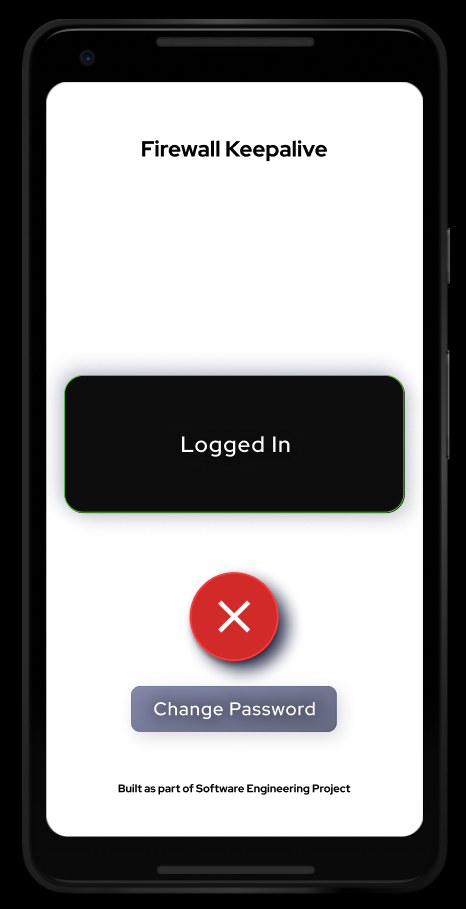
\includegraphics[scale=0.3]{images/hello2.png}

\subsection{Functional Requirements}

\begin{itemize}
\item \textbf{Purpose} : The Logout then logouts from the network and informs the user of the status change.
\item \textbf{User} : Gets a Logout Page informing the user on successful logout.
\item \textbf{Input Data} : User taps logout button.
\item \textbf{Output Data} : 'Successful Logout' response from the network.
\item \textbf{Invariants} : Logout Status of System in the Network.
\item \textbf{Pre-Conditions} : The user is at the keepalive page.
\item \textbf{Post-Conditions} : The user recieves the status upon clicking logout button.
\item \textbf{Basic Flow} : The system upon recieving the user signal, then requests a logout through the network, informing that the user intends to logout of the network. The network then sends a 'Successful Logout' response informing the same.
\item \textbf{Alternative Flow} : The network responds with a login page which indicates that the system is not logged in. The system then informs the user of the login change and requests the user to try logging in again.
\item \textbf{Business Rules} : This feature lets the user login and logout properly.
\end{itemize}
\section{KeepAlive}
\subsection{Description and Priority}
The system sends a keepalive request at specific intervals of time to the network.
Priority = 2.
\subsection{Functional Requirements}
\begin{itemize}
    \item  \textbf{Purpose}: Extend the Login window beyond 40 minutes.
    \item \textbf{User}: The application interacts with the firewall.
    \item \textbf{Input Data}: keepalive URL.
    \item \textbf{Output Data}: Success / Failure.
    \item \textbf{Invariants}: Login State, USER table and Network table.
    \item \textbf{Pre-conditions}: User is logged into a Campus Firewall.
    \item \textbf{Post-condition}: Keepalive table updated.
    \item \textbf{Basic Flow}: Application must request KeepAlive URL to CNC.
    \item \textbf{Alternate Flow}: Report error.
    \item \textbf{Business Rules}: This leads to no timeout after 40 minutes in keepalive.
\end{itemize}
\section{Add, Delete or Edit Multiple User Accounts}
\subsection{Description and Priority}
This feature lets the system manage multiple credentials on a single device with operations such as add, remove and manage credentials, so that the system can potentially use multiple accounts to authenticate using the system.
Priority = 5.\\ \\
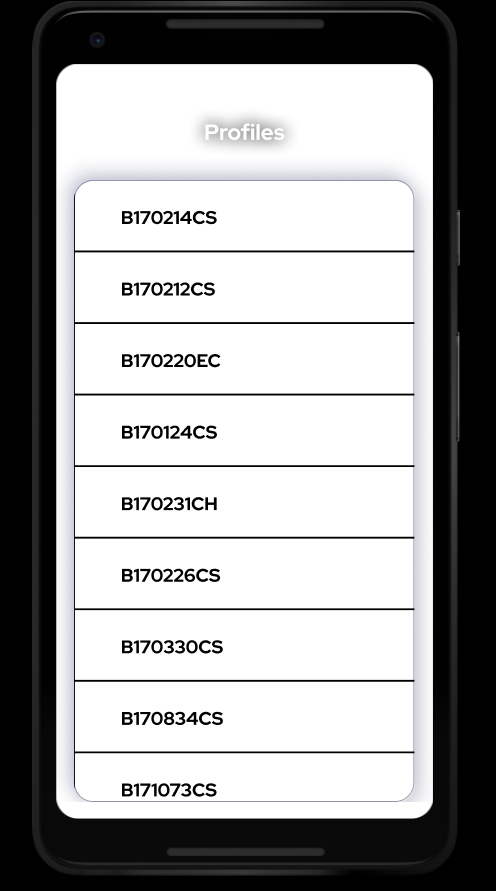
\includegraphics[scale=0.3]{images/list.png}
\subsection{Functional Requirements}
\begin{itemize}
    \item \textbf{Purpose} : To allow the user to manage (add, modify or remove) credentials.
    \item \textbf{User} : The user recieves a list of credentials to manage.
    \item \textbf{Input Data} : User clicking 'Add' or 'Remove' or 'Edit' on a certain user.
    \item \textbf{Output Data} : 'Add' Page, 'Edit' Page on a Credential, or list without the user.
    \item \textbf{Invariants} : Human Error (Unintentionally Clicking Edit/Remove)
    \item \textbf{Pre-Conditions} : List of Profiles (accessible by clicking 'Manage' from Home-Page)
    \item \textbf{Post-Conditions} : Page for Add/Edit or List, whichever is relevant.
    \item \textbf{Basic Flow} : The user clicks a button and the system responds properly.
    \item \textbf{Alternate Flow}: Report error.
    \item \textbf{Business Rules} : This allows the user to manage the credentials in a sane manner.
\end{itemize}

\section{Set Credential Preferences}
\subsection{Description and Priority}
This feature lets the user manage the preferences for multiple credentials using a page for editing the account preferences.
Priority = 5.

\subsection{Functional Requirements}
\begin{itemize}
    \item \textbf{Purpose} : To allow the modification of credential properties.
    \item \textbf{User} : The application sends preferences page to allow modifications.
    \item \textbf{Input Data} : User Proposed Modifications
    \item \textbf{Output Data} : Status on Accepting or Rejecting Proposed Credential Modifications
    \item \textbf{Invariants} : Input from User
    \item \textbf{Pre-Conditions} : The user selects a credential to change preferences.
    \item \textbf{Post-Conditions} : Page exits on accepting changes or notification on rejected changes.
    \item \textbf{Basic Flow} : The application first presents a UI to modify the credential properties, upon clicking 'Submit' the system checks the modifications upon accepting it the system updates the database to reflect the modifications, upon which the application goes back.
    \item \textbf{Alternative Flow} : The application on recieving unintended changes, stops execution following which the system stops execution and informs the user of wrong information.
    \item \textbf{Business Rules} : This allows the user to change the account preferences.
\end{itemize}

\section{Log Keepalive History}
\subsection{Description and Priority}
This feature lets the system keep a keepalive history so that the system can potentially manage login and logout process better and also to keep track of any problems the app might act on, which could be used to also debug the software.
Priority = 2.
\subsection{Functional Requirements}
\begin{itemize}
    \item \textbf{Purpose}: It keeps a keepalive history which indicates which tracks and logs all the status changes of the system.
    \item \textbf{User}: The Application undergoes a change in keepalive state.
    \item \textbf{Input Data}: Signal Log for Keepalive Database.
    \item \textbf{Output Data}: Response on recording the log.
    \item \textbf{Invariants}: Login Status, Credential Preferences, Database Status
    \item \textbf{Pre-Conditions}: The Database for the Authentication has been set.
    \item \textbf{Post-Conditions}: The Database logs the Status Change (Login/Logout) for the system.
    \item \textbf{Basic Flow}: The system recieves the signal for the log change. The system then adds a log in the database logging in detail the change in log status and then returns back to respond with confirmation on return.
    \item \textbf{Alternative Flow}: The system upon recieving the signal, if does not find a valid database, then informs the user by the use of the application's notification system to notify the user that the database was not working properly, and then given a way to contact us for modifications.
    \item \textbf{Business Rules}: This allows the applications to work efficiently and properly.
\end{itemize}


\chapter{Other Nonfunctional Requirements}
\label{Other Nonfunctional Requirements}

\section{Performance Requirements}
FLMI is a light application that needs very few system resources to work. It is designed not to delay the system from other key processes and the response time of the program is immediate. Performance might be affected when the application has to check through multiple user accounts to find a valid login id.

\section{Safety Requirements}
The application is open-source, and its source code is freely available on GitHub. Any bugs or issues can be raised on the repository page. The community fixes those bugs and issues on its next release cycle.

\section{Security Requirements}
FLMI requires write access to the android SQLite database to store the user account details. Passwords of the users are saved to a database in the mobile device storage. The user's KeepAlive history is stored in the database of the mobile device.

\section{Software Quality Attributes}
FLMI has a well defined and easy to use interface it can be used by both experts and typical users. However, users must already have a basic knowledge of the Android UI before using it.

%\chapter{Other Requirements}
%\label{Other Requirements}

% Add this in assumptions and dependencies
%The application requires to be connected to the same wifi network without which if logged in the user is locked in that network and would be unable to log out until he goes back to the same network. That is the only other requirement that is required.

\begin{appendices}
\chapter{Glossary}
\begin{itemize}
    \item \textbf{Software Requirements Specification}: A software requirements specification (SRS) is a description of a software system to be developed.The software requirements specification lays out functional and non-functional requirements, and it may include a set of use cases that describe user interactions that the software must provide to the user for perfect interaction.
    
    \item \textbf{GNU General Public License}: The GNU General Public License (GNU GPL or GPL) is a widely-used free software license that guarantees end users the freedom to run, study, share, and modify the software.
    
    \item \textbf{GitHub}: GitHub is a global company that provides hosting for software development version control using Git. It offers all of the distributed version control and source code management (SCM) functionality of Git as well as adding its own features. It provides access control and several collaboration features such as bug tracking, feature requests, task management, and wikis for every project.
    
    \item \textbf{Free and open-source software}: Free and open-source software (FOSS) is software that can be classified as both free software and open-source software.[a] That is, anyone is freely licensed to use, copy, study, and change the software in any way, and the source code is openly shared so that people are encouraged to voluntarily improve the design of the software
    
    \item \textbf{Android}: Android is a mobile operating system based on a modified version of the Linux kernel and other open source software, designed primarily for touchscreen mobile devices such as smartphones and tablets.
    
    \item \textbf{APK}: Android Package (APK) is the package file format used by the Android operating system for distribution and installation of mobile apps and middleware.
    
    \item \textbf{network}: A network is a set of nodes connected by communication links. A node can be a computer, printer, or any other device capable of sending or receiving data from the other node through the network
    
    \item \textbf{WiFi}: Wi-Fi  is a family of wireless networking technologies, based on the IEEE 802.11 family of standards, which are commonly used for local area networking of devices and Internet access.
    
    \item \textbf{firewall}: A firewall is a network security system that monitors and controls incoming and outgoing network traffic based on predetermined security rules.A firewall typically establishes a barrier between a trusted internal network and untrusted external network, such as the Internet.
    
    \item \textbf{database}: Database is an organized collection of data, generally stored and accessed electronically from a computer system. Where databases are more complex they are often developed using formal design and modeling techniques.

\end{itemize}

%\chapter{Analysis Models}
%\chapter{To Be Determined List}


\end{appendices}





%%%%%%%%%%%%%%%%%%%%%%%%%%%%%%%%%%%%%%%%%%%%%%%%%%%%%%%%%%%%%%%%%%%%%%%%%%%%%%%%%
%% Source defintions
%%%%%%%%%%%%%%%%%%%%%%%%%%%%%%%%%%%%%%%%%%%%%%%%%%%%%%%%%%%%%%%%%%%%%%%%%%%%%%%%%
% When no use outcomment
%\bibliographystyle{alpha}

\renewcommand\bibname{References}
\bibliography{base/sources}


%%%%%%%%%%%%%%%%%%%%%%%%%%%%%%%%%%%%%%%%%%%%%%%%%%%%%%%%%%%%%%%%%%%%%%%%%%%%%%%%%
%% Inserting the appendix
%%%%%%%%%%%%%%%%%%%%%%%%%%%%%%%%%%%%%%%%%%%%%%%%%%%%%%%%%%%%%%%%%%%%%%%%%%%%%%%%%
% When no use outcomment
%\newpage
\appendix 
% Adds appendix as chapter to toc
\addcontentsline{toc}{chapter}{Appendix}


\chapter{First}


\chapter{Second}


\end{document}*/***********************************************************************8	
